% Chapter 2

\chapter{Research definition} % Main chapter title

\label{Chapter2} % For referencing the chapter elsewhere, use \ref{Chapter1} 

%----------------------------------------------------------------------------------------
\section{The practical problem}
\label{the_practical_problem}

Defining a method to quantify the evolution of forks would mean that forking is no more a step in the dark, but instead could become a powerful tool for solving recurring problems of software development. The practical problem was examined here by answering two research questions:

\definition{Research Question 1}{Can a threshold be determined beyond which two diverging development branches will be more likely to fork than to merge?}

\noindent
If forking is a risk \citep{Kogut2001a}, then knowing whether a fork is about to happen can facilitate the choice of a contingency strategy. A metric of the dissimilarity between parallel development strands could detect whether development is about to cross a threshold beyond which a fork will be unavoidable. The value of this threshold can be approximated by examining the release history of well-known forks.

\definition{Research Question 2}{Can the likely outcome (cooperation, competition or discontinuation) of an ongoing fork be predicted?}

\noindent
\citet{Nyman2013a} argue that the right to fork inherent in open source licenses explains the resilience and innovation potential of the open source sector, however this potential can only be released if an ongoing fork is heading in the right direction, i.e. if separate teams are cooperating on a shared code base. Forks with known different outcomes: competition (e.g. MySQL/MariaDB), cooperation (e.g. Linux/Android), discontinuation of a branch (e.g. OpenOffice/LibreOffice) can be examined to answer the second research question.

%----------------------------------------------------------------------------------------

\section{Existing relevant knowledge}

This literature review is structured as follows: (2.2.1) software metrics, (2.2.2) evolution of software systems, (2.2.3) relevant evolutionary techniques, (2.2.4) software forks as risk or opportunity, (2.2.5) application of methods from evolutionary biology to software evolution.

\subsection{Software metrics}
\label{software_metrics}

\citet{Nagappan2008a} differentiate between methods for quantifying code structure and methods for quantifying organizational structure and evaluate the applicability of these methods for predicting fault-proneness of individual software components. As forking has technical and organizational aspects, the organizational metrics introduced by the authors are especially relevant. The purpose of \citet{Nagappan2008a} is different from the problem at hand; however, their comprehensive overview of software metrics and their rationales can provide guidance on which metrics to choose for data collection.

\noindent
\citet{Nagappan2008a} list the following metrics for quantifying code structure:

\begin{itemize}
  \item{“Code churn” is a measure of all the changes to a code base throughout its history.}
  \item{“Code complexity” is primarily relevant to object-oriented software and is obtained from the number of methods and inheritance depth of each class.}
  \item{“Code dependencies” measures how much the software depends on external components.}
  \item{“Code coverage” examines the percentage of code covered by automated tests.}
\end{itemize}

\noindent
\citet{Nagappan2008a} list the following metrics for quantifying organizational structure:

\begin{itemize}
  \item{“Number of engineers” and “Number of ex-engineers” are measures of how much knowledge remains in the team and how much has been lost.}
  \item{“Edit frequency” counts the number of changes contributed by each engineer.}
  \item{“Depth of ownership” tries to quantify at which organizational level the decisions concerning the software are being taken.}
  \item{“Percentage of organization contributing to development” and “Organizational code ownership” attempt to measure the communication overhead resulting from development inside an organization.}
  \item{“Organizational code ownership” measures the diversity of contributors.}
\end{itemize}

\subsection{Evolution of software systems}
An early attempt to describe the software maintenance process as evolution can be credited to \citet{Lehman1980a}. In this insightful paper, \citet{Lehman1980a} postulates that there are recurring patterns which govern software evolution, independently of the decisions taken by individual managers and programmers. These patterns are colloquially known as "Lehman's laws". Particularly the third law: "The Fundamental Law of Program Evolution" is of interest here, as it describes the software process as a self-regulating system, composed not only of the source code, but also of the organizations, managers, programmers and users involved. Through a case study, \citet{Lehman1980a} gathers empirical evidence for his hypothesis. This paper pioneers at least three interesting points: software evolves through constant interaction with its environment, the software production process is a self-regulating system, and quantitative analysis can improve project planning.

\citet{Nehaniv2006a} concentrate on the differences between biological and software evolution. This paper shows the limits of the “software evolution” metaphor: studies on software evolution are yet to agree on a clear-cut definition of what constitutes a population, an individual, a species or heritable characteristics in a software context. \citet{Yu2006a} concentrate on evolutionary aspects common to biological systems and software systems and try to delineate solutions for the issues raised by \citet{Nehaniv2006a}. \citet{Yu2006a} maintain that if the term “software system” is defined so as to include a system's infrastructure, code base and community of developers, then a software system is capable of sustaining itself and therefore the term evolution is applicable.

\subsection{Relevant evolutionary techniques}
The field of taxonomy is concerned with classifying organisms based on their observable characteristics; by contrast, the field of cladistics is concerned with reconstructing biological lineages \citep{Rohlf2013a}. A third approach, phylogenetics, seeks to unravel the mechanisms responsible for the diversity of lineages \citep{Garamszegi2014a}. These fields have in common that they apply statistical methods to generate hypotheses about the evolutionary relationships of populations. These hypotheses are commonly presented using phylogenetic trees \citep{Baum2008b}.

Among the methods available for estimating phylogenetic trees, “distance matrix methods”, i.e. methods that use a matrix of pairwise dissimilarity between observable characters, have been found to produce accurate results \citep{FelsensteinJ.andFelenstein2004a} and to perform well on large data sets \citep{Desper2005a}. One of the earliest distance matrix methods, “Unweighted Pair Group Method with Arithmetic Mean” (UPGMA), can be traced back to the work of Sneath and Sokal on numerical taxonomy during the 1960's. In a paper published in the influential magazine Nature, \citet{Sneath1962a} outline the principles underlying UPGMA: organisms presenting a high proportion of common characters are grouped together using statistics and all characters are considered equal in weight. This constitutes a departure from taxonomical practice hitherto, where classification was based on the presence of particular features selected by a taxonomist. The principal claim of the authors is that the statistical nature of numerical taxonomy guarantees the objectivity and repeatability of the classification.

Distance methods estimate a phylogenetic tree by computing a matrix of pairwise dissimilarity between the entities to be classified, and then applying a classification algorithm to the matrix. However, a matrix can theoretically result in multiple trees, and the choice of algorithm affects the topology of the resulting tree \citep{Paradis2011}. Using a computer is a prerequisite for applying these techniques and several software libraries help to achieve this goal. \citet{Paradis2011} provides up-to-date guidance on how to store, handle and analyse phylogenetic data using the R-language for statistical computing.

\subsection{Software forks as risk or opportunity}
\citet{Kogut2001a} maintain that software development under an open source licensing regime is more efficient than under strong intellectual property rights, and that the resulting community-based cooperation is more efficient than in-house competitive development. By examining the development processes in two open source projects: the Linux kernel and the Apache web server, \citet{Kogut2001a} conclude that governance structures in open source projects are shaped by the need to ward off the risk of forking. Additionally, the authors relate the often modular structure of open source programs to this very risk. Kogut and Metiu deduce that forking is the major risk faced by open source development, and that forking must be avoided as otherwise the community of developers would fragment and the project would lose the competitive edge it gained through open source licensing. This paper provides evidence for considering forks as risks.

\citet{Nyman2013a} adopt the opposite view. They argue that forking is not intrinsically negative, a synonym for wasted resources, incompatible versions and a risk to the continuation of a project. On the contrary, they see the liberty to fork, which is inherent in open source licenses, as a remedy to recurring problems of proprietary software: planned obsolescence, "hijacked" projects etc. Additionally, \citet{Nyman2013a} discuss business models built around forks. These are able to thrive in what the authors call a software ecosystem, and are facilitated by a thorough knowledge of the possibilities of open source licenses. Nyman and Lindman's paper does not provide in-depth case studies or a systematic review. The authors make a contribution to the study of forks nonetheless, by placing the practice of forking within a wider technological, managerial and economical context. This paper sets the background for considering forks as opportunities.

\citet{Robles2012a} conduct a comprehensive study of software forks. This paper provides a definition of forking and statistics regarding the relative frequency of forks, their reasons and outcomes.

\subsection{Application of methods from evolutionary biology to software evolution}
A search for the keywords “software fork”, “cladistics”, “phylogenetic” and “taxonomy” in the Open University library, the Basel Academic Search Engine and Google Scholar yielded no relevant articles, therefore to my knowledge, no study to date links evolutionary techniques to software forking. However, several researchers have studied the application of methods from evolutionary biology to different areas of software evolution.

\citet{Tenev2012a} study the evolution of six open source operating systems of the BSD family. \citet{Tenev2012a} use algorithms from biological genetics to study the similarity between lines of source code. They propose a new algorithm that can detect similarities of source code, even when files have been renamed or moved. Their algorithm is based on techniques used in genetics; however, they do not present a clear-cut solution to the problem of what constitutes a gene in a software context, a problem raised by \citet{Nehaniv2006a}. Additionally, their study is limited to characteristics of the code base, and they do not consider any team characteristics.

Nevertheless, \citet{Tenev2012a} are able to construct relatively simple evolutionary trees and claim that these trees represent the correct evolution of the BSD family, although it remains unclear how this claim can be substantiated.

\citet{Benlarabi2015b} attempt a 'cladistic' approach to the study of variants in a software product line. Software variants are produced by cloning and customizing existing software, within the limits of a common platform. Their study aims at predicting future changes and user requirements. \citet{Benlarabi2015b} use the functional features of each software variant as characters. They encode the presence or absence of each feature in a matrix and construct a phylogenetic tree by using clustering. \citet{Benlarabi2015b} use three measures to analyse the trees: the number of shared features, the distance between variants and the number of derived products from each variant. Although the choice of characters used by \citet{Benlarabi2015b} is an interesting approach, they limit themselves to using a general hierarchical clustering algorithm and therefore do not exploit the full potential of phylogenetic methods.

%----------------------------------------------------------------------------------------

\section{Objectives}

As specified in paragraph \ref{aim}, the aim of this research was to gain empirical evidence of whether phylogenetic methods from evolutionary biology can quantify the risks and opportunities associated with software forking processes. It was sought to achieve this aim by answering the two research questions specified in paragraph \ref{the_practical_problem}. It was attempted to answer these research questions by pursuing the objectives shown in the goal diagram in figure \ref{fig:objectives} and described below.

\begin{figure}[H]
  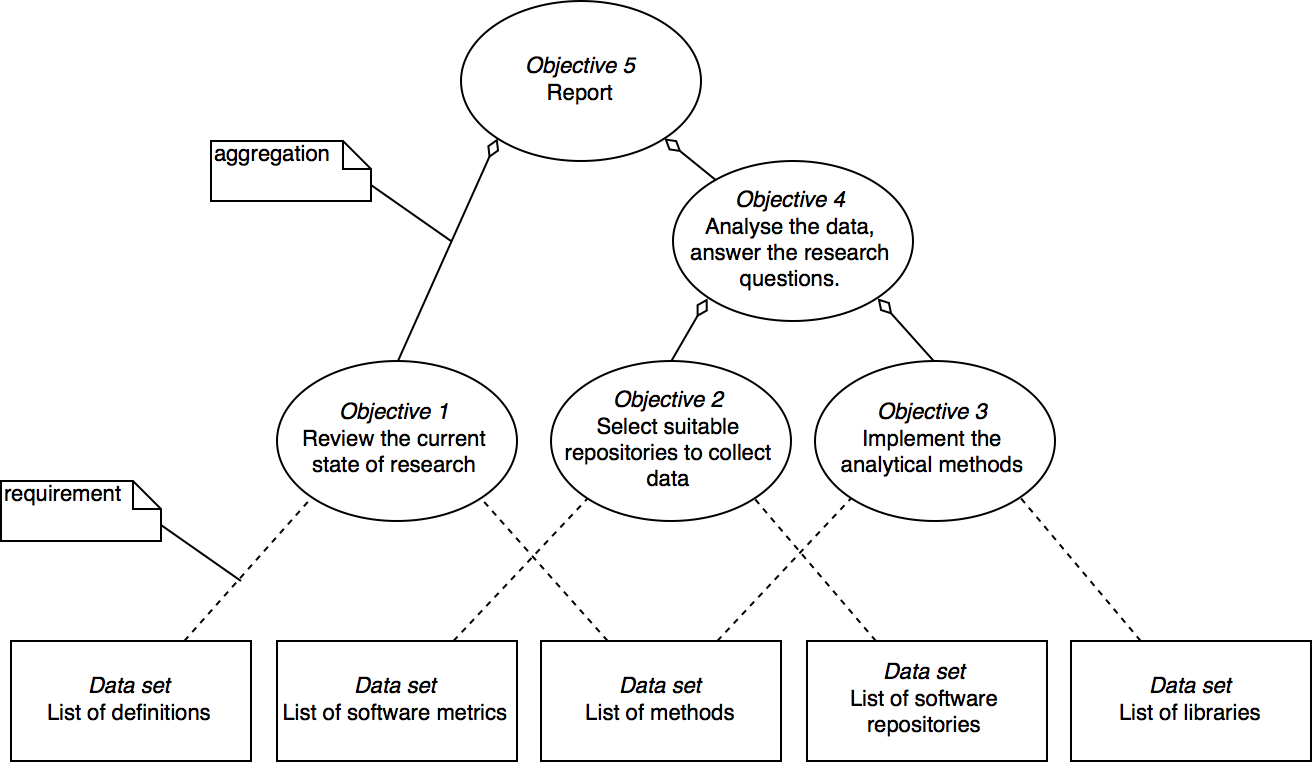
\includegraphics[width=\textwidth]{objectives_questions_and_data.png}
  \caption{Model of objectives and data sets required.}
  \label{fig:objectives}
\end{figure}

\begin{table}[H]
\caption*{Objective 1: Review the current state of research.}
\label{table:objective1} 
\centering
\begin{tabu} to \linewidth{p{5cm} p{5cm} p{5cm}}
\toprule
Task & Dataset & Method \\
\midrule
Attempt a working definition of the terms "fork" and “software evolution”. & A list of definitions. & Literature review \\
\midrule
Select methods from evolutionary biology. & A list of methods. & Literature review \\
\bottomrule
\end{tabu}
\end{table}

\begin{table}[H]
\caption*{Objective 2: Select suitable repositories to collect data.}
\label{table:objective2}
\centering
\begin{tabu} to \linewidth{p{5cm} p{5cm} p{5cm}}
\toprule
Task & Dataset & Method \\
\midrule
Select metrics applicable to software forks. & A list of software metrics. & Literature review \\
\midrule
Select suitable repositories and collect data. & Required or interesting repository characteristics, a list of software metrics. & Literature review \\
\bottomrule
\end{tabu}
\end{table}

\begin{table}[H]
\caption*{Objective 3: Implement the analytical methods.}
\label{table:objective3}
\centering
\begin{tabu} to \linewidth{p{5cm} p{5cm} p{5cm}}
\toprule
Task & Dataset & Method \\
\midrule
Select software libraries. & A list of libraries. & Literature review \\
\midrule
Implement the software & A list of methods. & Documentation review \\
\bottomrule
\end{tabu}
\end{table}

\begin{table}[H]
\caption*{Objective 4: Analyse the data using methods from evolutionary biology. Answer the research questions.}
\label{table:objective4}
\centering
\begin{tabu} to \linewidth{p{5cm} p{5cm} p{5cm}}
\toprule
Task & Dataset & Method \\
\midrule
Answer RQ1 & Data collected (objective 2), set of analytical methods (objective 3) & Estimate phylogenies for each fork case. Analyse. \\
\midrule
Answer RQ2 & Data collected (objective 2), set of analytical methods (objective 3) & Estimate phylogenies, obtained from different character sets. Analyse. \\
\bottomrule
\end{tabu}
\end{table}

\begin{table}[H]
\caption*{Objective 5: Report}
\centering
\begin{tabu} to \linewidth{p{5cm} p{5cm} p{5cm}}
\toprule
Task & Dataset & Method \\
\midrule
Report recommendations for practitioners. & The current state of research (objective 1), the results of the analysis (objective 4) & Compile and present an account. \\
\bottomrule
\end{tabu}
\end{table}

%----------------------------------------------------------------------------------------

\section{Summary of Chapter 2}
The concept of evolution has been used at least since 1980 in a software development context. Moreover, there is an abundant body of work on statistical methods for quantifying and describing biological evolutionary processes. However, although quantitative methods have been used to facilitate project management in different use cases, such as predicting fault-proneness of software, no work was found which applies biological evolutionary techniques to quantify the evolution of software forks. Therefore, primary research was required to answer the research questions specified in paragraph \ref{the_practical_problem}. In order to carry out this research, 5 objectives were defined: reviewing the current state of research, selecting suitable open source repositories to collect data about forks, porting methods from evolutionary biology to analyse the data acquired from the repositories, and reporting the results for an audience of practitioners.

